\chapter{Описание моделей динамики исполнительных механизмов ДРК}\label{ch:Propulsion}

Исполнительные механизмы ДРК определяют эффективность траекторного маневрирования НПА, а также возможность его динамического позиционирования в точке или зависания в толще воды.
На практике используются различные конструктивные схемы ДРК, в состав которых могут входить маршевые и подруливающие движители, носовые и кормовые рулевые устройства.

Наиболее распространенными типами движителей являются гребные винты в насадке и водометные движители, которые могут устанавливаться стационарно на корпусе аппарата или на поворотных кронштейнах, которые поворачиваются на требуемый угол в плоскости или пространстве для изменения направления действия силы тяги.
При этом использование водометных движителей ограничено их сравнительно низким КПД (0.5–0.55) по сравнению с гребными винтами, у которых он может достигать значений 0.7–0.75 \cite{инзарцев2018подводные}. Гораздо меньший КПД имеют такие экзотические движительные установки, как крыльчатые, волновые или машущие. 

Рулевые устройства, использующие гидродинамические крылья в качестве исполнительного органа, как известно, имеют низкую эффективность при малых скоростях набегающего потока \cite{агеев2015авто}.
При этом на крейсерских скоростях движения использование носовых и кормовых рулей направления и глубины имеет очевидное преимущество по сравнению с подруливающими движителями в части энергопотребления.
Остановимся на традиционных исполнительных элементах ДРК многофункционального НПА, обеспечивающего выполнение обзорно-поисковых работ с движением в широком диапазоне скоростей хода и динамическое позиционирование в толще воды.

Для корректного и энергетически эффективного решения задачи распределения управляющего воздействия на исполнительные механизмы движительно-рулевого комплекса необходимо корректно статически описать как сам комплекс исполнительных механизмов, так и динамические процессы происходящие в них с учётом гидродинамических особенностей их поведения.

\section{Модель маршевого движителя ПА}
Это один или несколько кормовых движителей, обеспечивающих продольное движение аппарата, а также возможность маневрирования по глубине и курсу.

В работе \cite{10.1109/48.107145} была предложена модель движителя заданная в форме пространства состояний по входному параметру $n$ где $n$ -- скорость вращения вала:
\begin{gather}
    \label{eq:thruster_dynamic_1}
    J_m\dot{n} + K_{n|n|}n|n| = Q \\
    T = T(n, u_p)
\end{gather}

\noindent где:
\begin{itemize}
    \item $Q$ -- момент сопротивления вращению на валу привода;
    \item $J_m$ -- момент инерции на привода/пропеллера (кг$\cdot$м$^2$);
    \item $K_{n|n|}$ -- нелинейный коэффициент демпфирования мотора (кг$\cdot$м$^2$);
    \item $u_p$ -- скорость потока в канале движителя;
\end{itemize}

Коэффициент $K_{n|n|}$ определяется следующим образом:
\begin{gather}
    K_{n|n|} = \frac{1}{2}\eta^3 \cdot p^3 \cdot \rho \cdot A \\
    J_m = \eta^2 \cdot p^2 \cdot \rho \cdot V
\end{gather}
где:
\begin{itemize}
    \item $\eta$ -- безразмерный коэффициент эффективности винта;
    \item $p$ -- шаг винта (продольное расстояние которое винт за один оборот), (pitch);
    \item $A$ -- площадь сечения винта, (duct area);
    \item $V$ -- объем насадки в которой расположен винт.
\end{itemize}

Позже модель, представленная уравнением \ref{eq:thruster_dynamic_1}, была усовершенствована в работе \cite{10.1109/48.468242} на основе исследований \cite{cody1992experimental, mclean1991dynamic}.
Новая модель описывает вектором из двух состояний и записывается следующим образом:
\begin{gather}
    J_m\dot{n} + K_{n|n|}n|n| = Q_m- Q \\
    m_f \dot{u_p} + d_f(u_p-u) |u_p - u| = T \\
    T = T(n,u_p) \\
    Q = Q(n,u_p)
\end{gather}
\noindent где:
\begin{itemize}
    \item $Q_m$ -- момент на валу сформированный приводом (Нм);
    \item $m_f$ -- масса воды захватываемая винтом (кг);
    \item $d_f$ -- квадратичный демпфирующий коэффициент (кг/м);
    \item $u$ -- продольная скорость движения ПА.
\end{itemize}

Экспериментальная проверка обоих подходов была проведена в работе \cite{whitcomb1999development}.

Кроме того, в работе \cite{blanke2000dynamic} рассматривается трехэтапная модель винта, которая уже учитывает упрощённую модель ПА для более точного расчета скорости потока набегающего на грибной винт:
\begin{gather}
    J_m\dot{n} + K_{n|n|}n|n| = \tau - Q \\
    m_f \dot{u_p} + d_{f0}u_p + d_f|u_p|(u_p - u_a) = T \\
    (m - X_{\dot{u}})\dot{u} - X_u u - X_{u|u|}u|u| = (1-t)T\\
    T = T(n,n_p) \\
    Q = Q(n,n_p)
\end{gather}

Последние исследования в области описания динамики движителя представлены в работе \cite{10.1109/robot.2005.1570115}.

Кроме того, разумно рассмотреть декомпозицию задачи и независимо рассмотреть стационарнуб модель гребного винта и модель динамики электрического привода.

\subsection{Модель гребного винта}

Для гребного винта с фиксированным шагом, момент на валу $Q$ и сила (упор) вырабатываемая винтом $T$ зависит от продольной скорости движения аппарата $u$, скорости потока воды $u_a$, а так же скорости вращения винта $n$.
Кроме этого на работу движителя влияют нестационарные потоки и различные эффекты которые влияют на эффективность работы движителя.
В соответствии с работами \cite{newman2018marine, breslin1996hydrodynamics, carlton2018marine} к особо влияющим эффектам можно отнеси следующие:
\begin{itemize}
    \item всасывание воздуха;
    \item кавитация;
    \item эффект Вагнера при вращении винта у раздела сред;
    \item эффекты связанные с влиянием морских волн;
    \item эффект Куснера (срыв потока).
\end{itemize}

Приведенные факторы рассматриваются в основном в приложении к суднам.
Для движителей подводных аппаратов, которые большую часть времени погружены под воду, первыми тремя эффектами можно пренебречь.
Эффект Куснера связанный со срывом потока связан с высокоамплитудными переключениями сигнала управления движителем и им можно пренебречь.

Квазистационарное моделирование тяги и крутящего момента движителя обычно происходит в терминах кривых подъемной силы и момент сопротивления, которые возможно преобразовать в тягу и момент.
Подъемная сила и момент сопротивления обычно формируются через безразмерные коэффициенты упора $K_T$ и момента $K_Q$, которые рассчитываются на базе швартовых испытаний движителя.
В ходе этих испытаний формируются кривые зависимости упора и момента от скорости вращения вала движителя
\begin{gather}
\label{eq:propeler_model}
    K_T (J_0) = \frac{T}{\rho D^4 n |n|}, \:
    K_Q (J_0) = \frac{Q}{\rho D^5 n |n|}
\end{gather}
\noindent где $D$ -- диаметр винта, $\rho$ -- плотность воды, а $J_0$ представляет собой относительную поступь и определяется следующим уравнением:
\begin{equation}
    J_0 = \frac{u_a}{nD}
\end{equation}
\noindent где $u_a$ -- скорость окружающей воды (совпадает со скоростью движения аппарата в случае установившегося движения).

Численные расчеты коэффициентов $K_T$, $K_Q$ обычно проводят на натурных экспериментах в специальных бассейнах.
При этом, обычно, нестационарными эффектами пренебрегают.

В свою очередь, сами безразмерные коэффициенты $K_T$, $K_Q$ могут быть описаны как функции со следующими параметрами (\cite{oosterveld1975further}):
\begin{gather}
    K_T = f_1 \left( J_0, \frac{P}{D}, \frac{A_E}{A_0}, Z \right) \\
    K_Q = f_2 \left( J_0, \frac{P}{D}, \frac{A_E}{A_0}, Z, R_n, \frac{t}{c} \right) 
\end{gather}
\noindent где:
\begin{itemize}
    \item $P/D$ -- шаговое отношение винта;
    \item $A_E/A_0$ -- отношение площади винта к площади движителя;
    \item $Z$ -- количество лопастей винта;
    \item $R_n$ -- число Рейнольдса;
    \item $t$ -- максимальная толщина лопасти;
    \item $c$ -- длина хорды лопасти.
\end{itemize}

На основе уравнения \ref{eq:propeler_model} упор движителя и момент сопротивления может быть записан следующим образом:
\begin{gather}
    T = \rho D^4K_T(J_0)n|n| \\
    Q = \rho D^5K_Q(J_0)n|n|
\end{gather}

\subsection{Модель привода движителя}

Модель привода движителя обычно представляют следующим набором уравнений:
\begin{equation}
	\label{eq:motor_model}
	\begin{array}{ll}
	L_a\frac{d}{dt}i_m &=-R_ai_m-K_m n + V_m \\
    J_m\dot{n} &= K_m i_m - Q
	\end{array}
\end{equation}

\noindent где:
\begin{itemize}
    \item $V_m$ -- напряжение на обмотках привода (В);
    \item $i_m$ -- ток на обмотках привода (А);
    \item $n$ -- скорость вращения вала (об/с);
    \item $L_a, R_a$ -- индуктивность и сопротивление обмоток, соответственно;
    \item $K_m$ -- коэффициент крутящего момента мотора;
    \item $J_m$ -- момент инерции ротора.
\end{itemize}

Поскольку электрическая постоянная времени $T_a=L_a/R_a$ мала по сравнению с механической постоянной времени мотора, допустимо следующее предположение:
\begin{equation}
    \frac{L_a}{R_a}\frac{d}{dt}i_m \approx 0
\end{equation}
\noindent следовательно динамику движителя можно упростить до следующего состояния:
\begin{gather}
    \label{eq:motor_dynamics}
    0 = -R_a i_m-K_m w_m + V_m \\
    J_m\dot{n} = K_m i_m - Q
\end{gather}

При различных типах управления приводом, возможно представление его динамики в различной записи.

\subsection{Типы управления приводом движителя ПА}
\paragraph{Управление током}
Пусть реализовано линейное пропорциональное управление током на обмотках мотора, тогда задаваемое напряжение на обмотках будет представлено следующим выражением:
\begin{equation}
    V_m = K_p(i_d - i_m),\: K_p>0
\end{equation}
\noindent где $i_d$ -- целевое значение тока, тогда уравнение \ref{eq:motor_dynamics} будет преобразовано следующим образом:
\begin{equation}
    (R_a + K_p)i_m = -K_mn + K_pi_d
\end{equation}

А модель динамики привода будет представлена в виде:
\begin{equation}
    \label{eq:motor_dynamic_current}
    J_m\dot{n} + \frac{K_m^2}{R_a+K_p}n = \frac{K_m K_p}{R_a + K_p}i_d - Q
\end{equation}

В случае если $K_p \gg R_a > 0$, то выражение можно упростить:
\begin{equation}
    J_m\dot{n} = K_m i_d - Q  
\end{equation}

\paragraph{Управление моментом}
Для мотором постоянного тока, создаваемый им момент будет пропорционален току на обмотках, таким образом целевое значение момента $Q_d$ может быть записано следующим образом:
\begin{equation}
    Q_d = K_m i_d
\end{equation}

При такой записи, из уравнения \ref{eq:motor_dynamic_current} уравнение динамики для данного режима управления может быть получено сразу же:
\begin{equation}
    J_m\dot{n} + \frac{K_m^2}{R_a+K_p}n = \frac{K_p}{R_a + K_p}Q_d - Q
\end{equation}

В случае если $K_p \gg R_a > 0$, то выражение упращается аналогичным образом:
\begin{equation}
    J_m\dot{n} = Q_d - Q  
\end{equation}

\paragraph{Управление напряжением на обмотках}
Уравнение динамики при таком режиме управления приводом может быть получено на базе уравнений \ref{eq:motor_dynamics} следующим образом:
\begin{equation}
    J_m\dot{n} + \frac{K_m^2}{R_a}n = \frac{K_m}{R_a}V_m - Q
\end{equation}

\section{Особенности работы движителей подруливающего типа}
Описание работы подруливающего движителя описывается существенно более сложнее по сравнению с маршевым движителем за счёт особенностей взаимодействия создаваемой подруливающим движителем пропульсивной струи с корпусом подводного аппарата.
Научные труды посвященные гидродинамическим особенностям работы подруливающих движителей в первую очередь были проведены в рамках исследования эффективности движительно-рулевых комплексов судов \cite{chislett1966influence, english1964design, brix1973lateral}.
Кроме того, большое исследование данного вопроса было проведено в докторской диссертации \cite{nienhuis1992analysis}.
Общий вывод представленных работ и результатов натурных экспериментов заключается в том, что работа подруливающих движителей тунельного типа становится неэффективной на скоростях движения судов свыше 1–1,5 м/с \cite{english63}.

Первое исследование эффективности подруливающих движителей для АНПА была было проведено в работе \cite{saunders2002effect}. 
В рамках этой работы представлен полноценный анализ эффективности подруливающего движителя аппарата ``C-SCOUT'' для большого диапазона скоростей его движения и углов атаки в диапазоне $\pm90^{\circ}$.

Большое исследование эффективности работы подруливающих движителей АНПА с формированием обобщенной модели влияния скорости и направления набегающего потока на аппарат было проведено в рамках работы \cite{palmer2008modelling} а так же в последующей докторской работе этого же автора \cite{palmer2009analysis}.

В упомянутых научных работых было показано что падение эффективности подруливающего движителя не связано с уменьшеньем эффективности самого устроства, а скорее с взаимодействием пропульстивной струи, которую создает подруливающий движитель с набегающим на ПА потоком.

Работа подруливающего движителя ПА в случае если он находится в состоянии покоя полностью эквивалентна модели маршевого движителя, т.е. на аппарат действует определенная сила (упор) приложенная к точке крепления движителя за счет формирования пропульсивной струи ПА.
Но в случае, когда ПА движется с продольной скоростью $u$, то пропульсивная струя формируемая подруливающим движителем формирует гидродинамическую тень (на рисунке закрашена серым цветом) на корпусе ПА в области за подруливающей шахтой (рисунок \ref{fig:modelling-tunnel}).
За счет этого формируется разность давлений между различными областями ПА, которая, в свою очередь, формирует силу $F_S$ обратную по направлению силе создаваемой подруливающим движителем $F_T$.

\begin{figure}[ht]
    \centering
    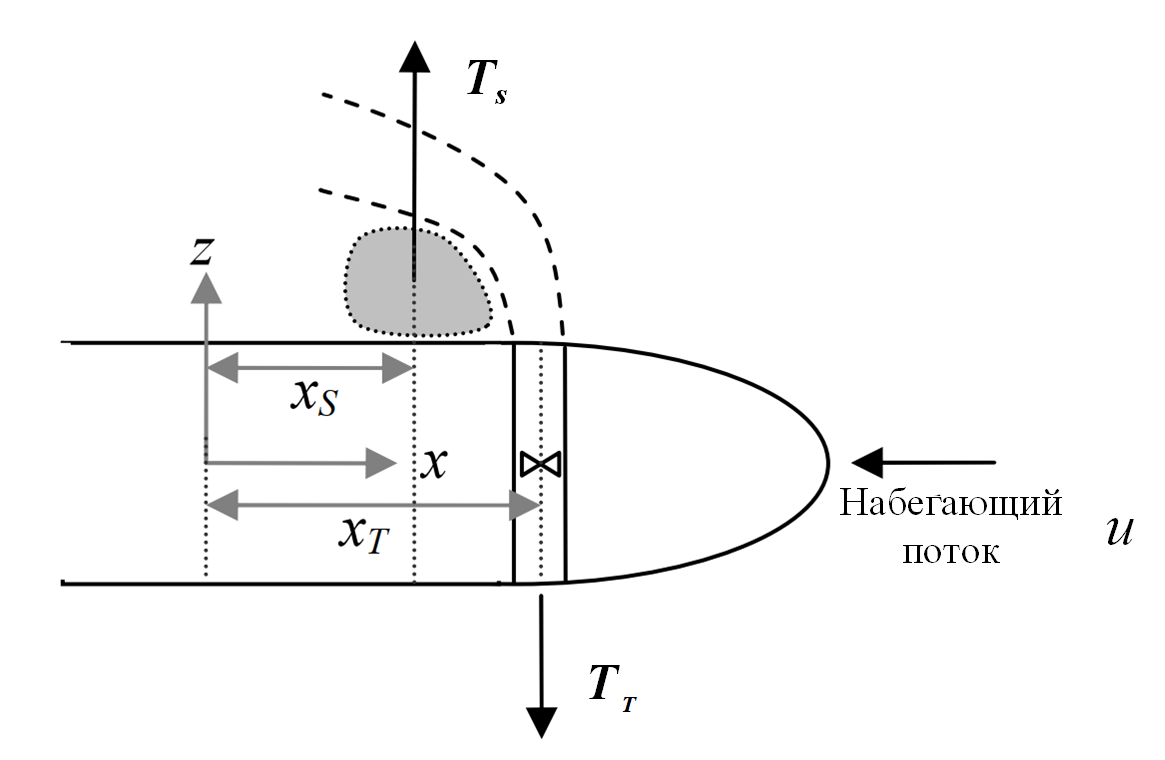
\includegraphics[width=0.8\linewidth]{modelling/Моделирование - подруливающий движитель силы.png}
    \caption{Особенности поведения подруливающего движителя в набегающем потоке.}
    \label{fig:modelling-tunnel}
\end{figure}

При низких и средних скоростях продольного движения ПА, когда формируемая подруливающим движителем скорость пропульсивной струи существенно выше скорости АНПА наклон струи незначителен, гидродинамическая тень мала и соответственно мала и сила создаваемая разностью давлений на корпус ПА.
При высоких скоростях движения ПА, когда скорость набегаемого на АПНА потока сопоставима или выше по скорости чем скорость создаваемой подруливающим движителем пропульсивной струи, её наклон существенно выше, как и создаваемая гидродинамическая тень и общая эффективность подруливающего движителя падает значительно.
Важно так же учитывать что с увеличением гидродинамической тени точка приложения разности давлений начинает сдвигаться и результирующий момент действующий на аппарат формируемый силой $F_S$ меняется.

При этом разница давлений вокруг входа в туннель подруливающего движителя и вокруг выходом из него не оказывают значительного влияния на эффективность подруливающего движителя \cite{brix1973lateral}.

Количественные изменения эффективности подруливающего движителя были проведены в работе \cite{chislett1966influence} в котором экспериментально исследовалась эффективность движительно-рулевого комплекса на макете судна.
В ходе эксперимента авторы получили коэффициенты эффективности упора $K_F$ создаваемого подруливающим движителем и момента сопротивления вращению гребного винта $K_N$.
Они определяются следующим образом:
\begin{equation*}
	K_F = \frac{T_{u/u_j}}{T_0}; \: K_N = \frac{N_{u/u_j}}{N_0}
\end{equation*}
\noindent где $T_{u/u_j}$ и $N_{u/u_j}$ упор и момент сопротивления вращению при набегающем потоке, а $T_0$ $N_0$ -- при его отсутствии.

\begin{figure}[ht]
    \centering
    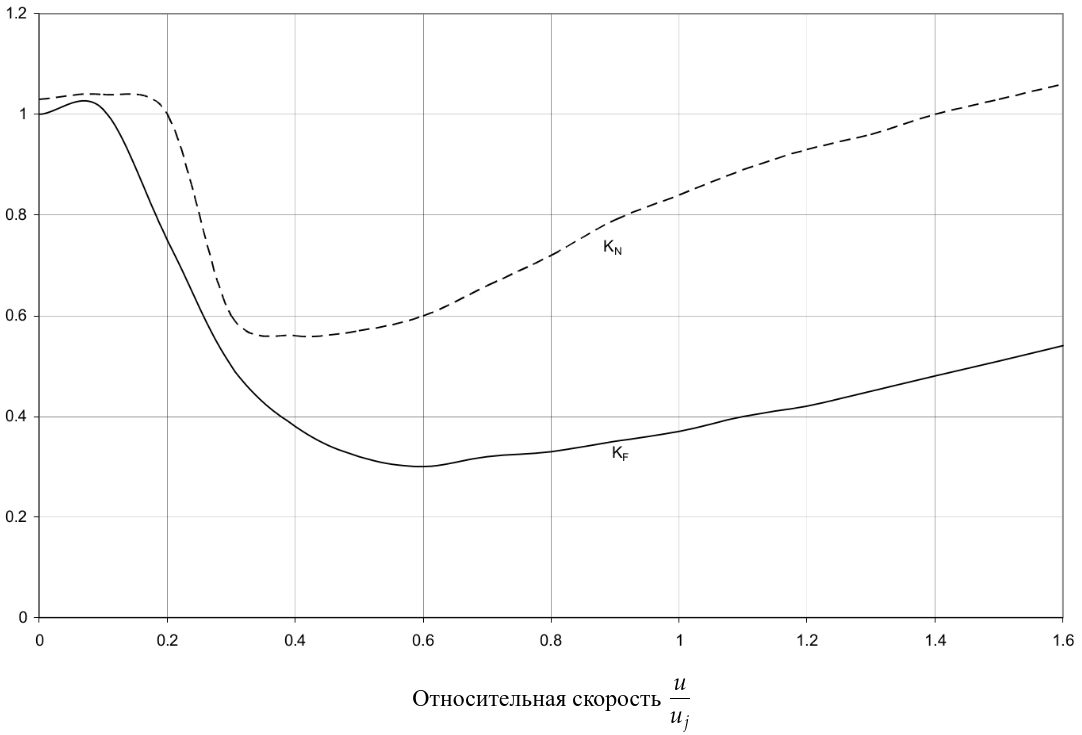
\includegraphics[width=0.8\linewidth]{modelling/Эксперимент - Kt Kn подруливающий движитель.png}
    \caption{Коэффициенты $K_F$, $K_N$ подруливающего движителя, полученные в ходе натурных экспериментов.}
    \label{fig:tunnel_effectivness}
\end{figure}

По рисунку \ref{fig:tunnel_effectivness} представленному в статье \cite{chislett1966influence} видно что результирующий упор создаваемый подруливающим движителем падает при большом отношении скорости набегающего потока к скорости пропульсивной струи, при этом как момент сопротивления вращению ГВ падает существенно слабее, т.е. эффективность работы подруливающего устройства становится крайне низкой.

Экспериментальные исследование эффективности подруливающего движителя для АНПА было так же проведено в работе \cite{beveridge1972design}, где были получены данные аналогичные представленным на рисунке \ref{fig:tunnel_effectivness}.

в работе \cite{palmer2009analysis} предложено силу формируемую разностью давлений представлять следующим образом:
\begin{equation*}
	T_S = T_T \exp \left[ -c \left( \frac{u}{u_j}^2 \right) \right]
\end{equation*}
\noindent где:
\begin{itemize}
	\item $T_S$ -- сила действующая на аппарат в связи с разностью давлений;
	\item $T_T$ -- упор создаваемый подруливающим движителем;
	\item $u$ -- скорость набегающего потока;
	\item $u_j$ -- скорость пропульстивной струи;
	\item $c$ -- некоторый коэффициент.
\end{itemize}

В свою очередь скорость пропульсивной струи, создаваемой работой подруливающего движителя может быть определена следующим уравнением:
\begin{equation*}
	u_j = \sqrt{\frac{T_T}{\rho A}}
\end{equation*}
\noindent где $\rho$ -- плотность воды, $A=\pi R^2$, где $R$ -- диаметр гребного винта подруливающего движителя.

Момент действующий на ПА формируемый упором движителя и гидродинамической силой определяется следующим образом:
\begin{equation*}
	M = F_T x_T + (F_T-F_S)x_S
\end{equation*}
\noindent где $x_T$ -- расстояние между ЦП подводного аппарата и точкой приложения силы $F_T$, а в свою очередь $x_S$ - это расстояние между ЦП ПА и точкой приложениия силы $F_S$, которая определяется следующим образом:
\begin{equation*}
	x_S = x_T - kD\frac{u}{u_j}
\end{equation*}
\noindent где $D$ -- диаметр туннеля подруливающего движителя, $k$ -- некоторый коэффициент.

Кроме величины набегающего потока на эффективность подруливающего движителя так же влияет угол атаки, т.е. разница между вектором скорости ПА и вектором скорости набегающего потока, которая возникает в случае несоосного течения или в ходе переходных процессов по курсу следования ПА.
В работе \cite{palmer2008modelling} представлена модель зависимости упора создаваемого подруливающим движителем от скорости набегающего потока и угла атаки.

\section{Модель рулевых устройств ПА}
В техническом отчете \cite{steenson2011control} подробно представлен расчет подъемной силы для АНПА ``Dolphin 2'', в котором ДРК состоит из четырех кормовых рулей нормального расположения и четырех подруливающих движителей (2-х вертикальных и 2-х горизонтальных).

Подъемная сила формируемая горизонтальными рулевыми устройствами в стационарном случае определяется следующим выражением:
\begin{equation}
    F_{lift} = \frac{1}{2}\rho v^2 A_{SP} C_{LSP}
\end{equation}
\noindent где:
\begin{itemize}
    \item $\rho$ -- плотность воды;
    \item $v$ -- скорость продольного движения АНПА;
    \item $A_{SP}$ -- площадь РУ;
    \item $C_{LSP}$ -- подъемный коэффициент РУ;
\end{itemize}

В свою очередь, подъемный коэффициент РУ $C_{LSP}$ быть расcчитан следующим образом:
\begin{equation}
    C_{LSP} = a_{sp}\alpha \left( \frac{2 \pi}{1 + (2/AR)} \right)
\end{equation}
\noindent где:
\begin{itemize}
    \item $a_{sp}$ -- коэффициент подъемной силы (1/$^\circ$);
    \item $\alpha$ -- угол поворота РУ относительно потока жидкости;
    \item $AR$ -- соотношение сторон РУ;
\end{itemize}

Соотношение сторон РУ $AR$ определяется следующим образом:
\begin{equation}
    AR = k \frac{S}{\bar{c}}
\end{equation}
\noindent где $S$ -- площадь РУ, $\bar{c}$ -- среднее значение длины РУ (chord), а коэффициент $k$ определяет влияние щели между РУ и корпусом ПА. Если щель отсутствует, то $k=2$, При отношении ширины щели к длине РУ около $0.1$ коэффициент $k\approx1.5$

Угол $\alpha$ определяет положение РУ относительно потока воды, в случае управления по глубине, можно эту переменную переписать следующим образом:
\begin{equation}
    \alpha = \delta - \theta
\end{equation}
\noindent где $\delta$ -- угол перекладки ГУ относительно ССК, $\theta$ -- текущий дифферент АНПА.

Традиционным конструктивным и эксплуатационным решением РУ является использование кормовых рулей и элеронов, хотя при малых скоростях движения находят применение и дополнительные рули глубины.
Управляющие моменты рулей являются функцией угла перекладки и скорости набегающего потока, при этом дополнительные силы лобового сопротивления не учитывается при анализе управления.
Модель РУ определяется следующими соотношениями \cite{боженов1986}:
\begin{equation}
	\label{eq:modelling-rudder}
	\begin{array}{ll}
    M_x^{rud} = m_x^{\delta} \cdot \delta_{\theta} \frac{\rho V^2}{2} U \\
    M_y^{rud} = m_y^{\delta} \cdot \delta_{\phi} \frac{\rho V^2}{2} U \\
    M_z^{rud} = m_z^{\delta} \cdot \delta_{H} \frac{\rho V^2}{2} U
    \end{array}
\end{equation}
\noindent где:
\begin{itemize}
    \item $M_x^{rud}, M_y^{rud}, M_z^{rud}$ -- управляющие моменты РУ по крену, курсу и дифференту, соответственно;
    \item $m_x^{\delta}, m_y^{\delta}, m_z^{\delta}$ -- производные гидродинамических характеристик от перекладки рулей крена, направления и глубины, соответственно;
    \item $\delta_{\theta}, \delta_{\phi}, \delta_{H}$ -- углы перекладки рулей крена, направления и глубины, соответственно;
    \item $U$ -- водоизмещение аппарата, м$^3$.
\end{itemize}

\section{Численное моделирование поведения исполнителнительных механизмов ДРК в набегающем потоке}
\subsection{Моделирование маршевого двигателя}
В рамках исследования необходимо определить насколько меняется поведение ИМ ДРК при движении АНПА в набегающем потоке.
Для численного анализа поведения маршевого движителя в набегающем потоке была разработана его блочная модель (рисунок \ref{fig:modelling-thruster}), где модель привода движителя описывается в соответствии с системой дифференциальных уравнений \ref{eq:motor_model}, а модель гребного винта - в соответствии с уравнениями \ref{eq:propeler_model}.
Параметры моделирования представлены в таблице \ref{tab:modelling-thruster}.

\begin{figure}[ht]
    \centering
    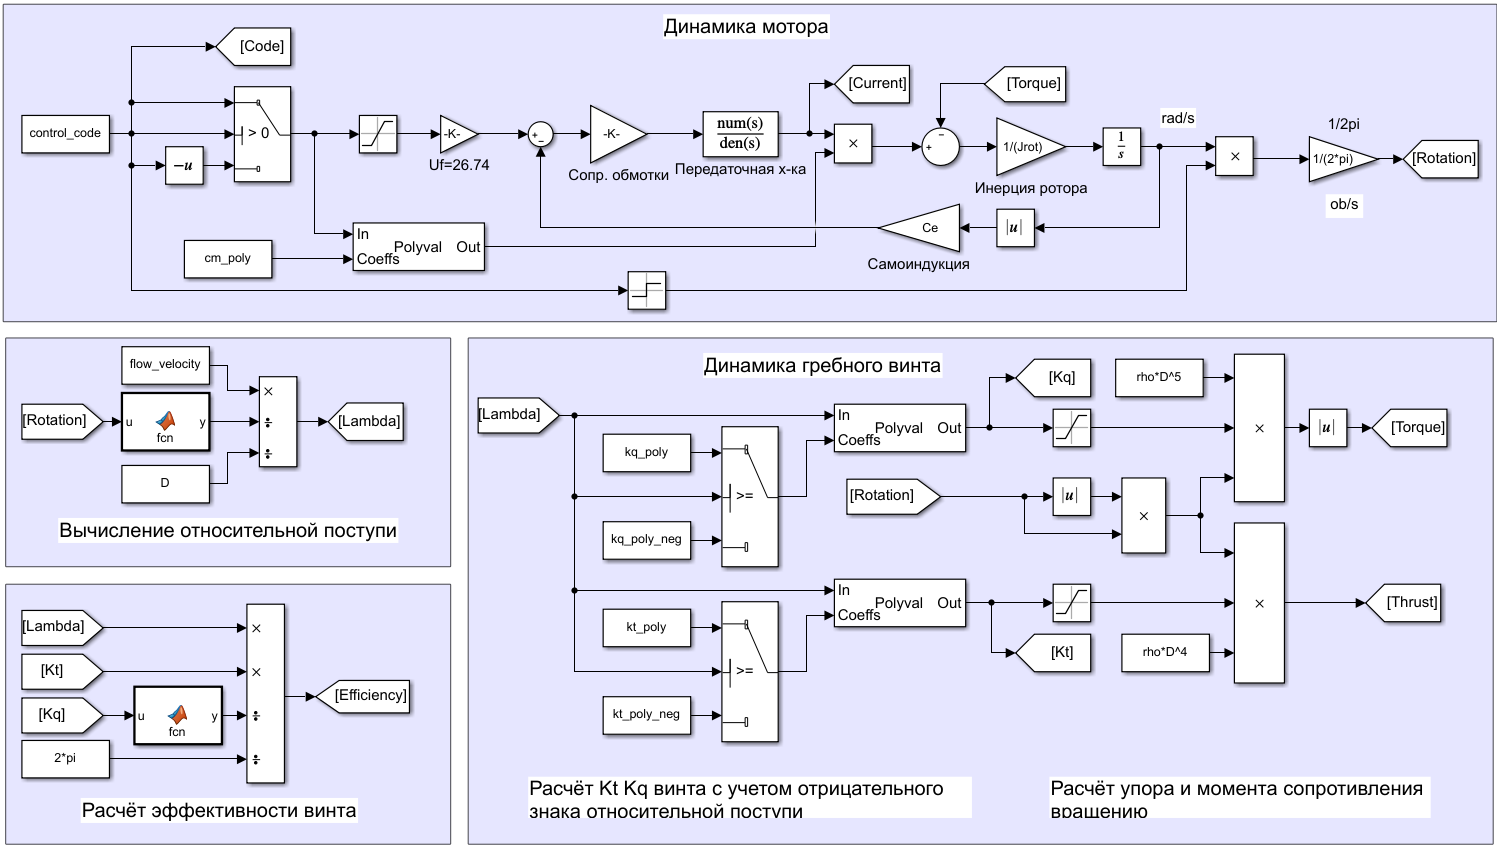
\includegraphics[width=1.0\linewidth]{modelling/Моделирование - маршевый движитель схема.png}
    \caption{Блочно-визуальная модель численного моделирования маршевого движетеля ПА.}
    \label{fig:modelling-thruster}
\end{figure}

\begin{table}
    \caption{Параметры моделирования движителя ПА.}
    \label{tab:modelling-thruster}
    \centering
    \begin{tabular}{lll}
        \toprule
        \makecell[l]{Наименование \\ параметра} & \makecell[l]{Идентификатор \\ в блочной модели} & Значение \\
        \midrule
        \multicolumn{3}{c}{Параметры ГВ} \\
        \midrule
        Диаметр, м  & D & 0,19\\
        Коэф. $K_T$ & kt\_poly & $-0.096\lambda^2 -0.277\lambda + 0.351$\\
        Коэф. $K_Q$ & kq\_poly & $-0.014\lambda^2 -0.030\lambda + 0.045$\\
        \midrule
        \multicolumn{3}{c}{Параметры электромотора} \\
        \midrule
        % Коэффициент момента, Н$\cdot$м/А & Km & 0,16\\
        Момент инерции ротора, кг$\cdot$м$^2$ & Jrot & 2,5$\cdot$10$^{-4}$ \\
        Сопротивление обмоток, Ом & Ranchor & 1,5 \\
        Электрическая постоянная, c & Tem & 0,0004 \\
        Коэффициент ЭДС, В/рад/с & Ce & 0,16 \\
        \bottomrule
    \end{tabular}
\end{table}

В рамках реализованной модели движителя был проведен анализ влияния соосного набегающего потока на упор создаваемый маршевым движителем при различных кодах управления (рисунок \ref{fig:modelling-thruster-velocity}), кроме того была явным образом расчитана зависимость упора создаваемого движителем от скорости набегающего потока для фиксированых значений кода управления (рисунок \ref{fig:modelling-thruster-code}).
Видно, что создаваемый упор существенно зависит от набегающего потока и при больших скоростях движения падает почти в 2 раза.

\begin{figure}[ht]
    \centering
    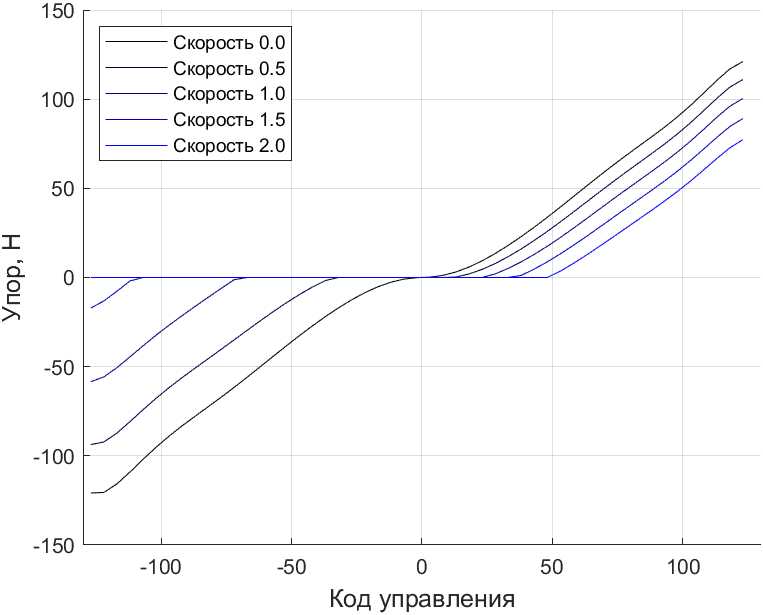
\includegraphics[width=0.8\linewidth]{modelling/Моделирование - маршевый движитель код.png}
    \caption{Численное моделирование упора создаваемого маршевым движителем при различных параметрах скорости набегающего потока.}
    \label{fig:modelling-thruster-velocity}
\end{figure}

\begin{figure}[ht]
    \centering
    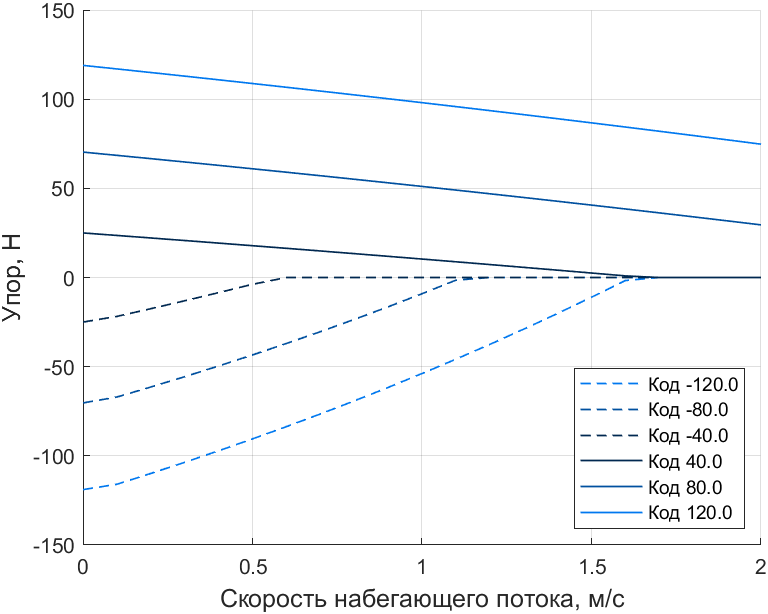
\includegraphics[width=0.8\linewidth]{modelling/Моделирование - маршевый движитель скорость.png}
    \caption{Численное моделирование упора создаваемого маршевым движителем при различных параметрах кода управления.}
    \label{fig:modelling-thruster-code}
\end{figure}

\subsection{Моделирование подруливающего двигателя}
В соответствии с моделью влияния набегающего потока на эффективность маршевого двигателя для численного анализа поведения подруливающего движителя была создана модель его блочная модель.
Все параметры модели движителя и гребного винта соответствуют параметрам указанным в таблице \ref{tab:modelling-thruster}.
Коэффицент подавления потока $C$ был принят с величиной 5.0.
В рамках реализованной модели подруливающего движителя был проведен численное моделирование влияния соосного набегающего потока на эффективное значение упор создаваемый подруливащим движителем при различных значениях набегающего потока (рисунок \ref{fig:modelling-tunnel-velocity})

\begin{figure}[ht]
    \centering
    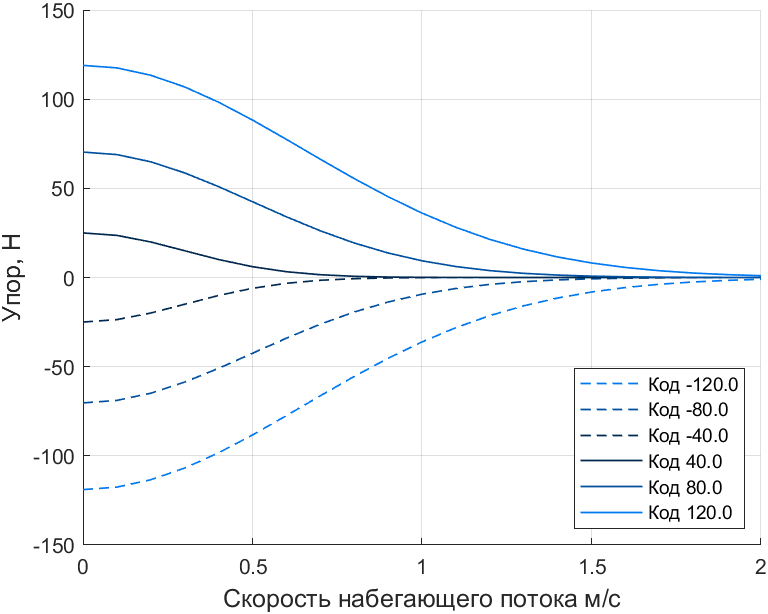
\includegraphics[width=0.8\linewidth]{modelling/Моделирование - подруливающий движитель скорость.png}
    \caption{Численное моделирование эффективного упора создаваемого подруливающим движителем при различных скоростях набегающего потока.}
    \label{fig:modelling-tunnel-velocity}
\end{figure}

\subsection{Моделирование руля управления ПА}
В соответствии с моделью руля управления (уравнение \ref{eq:modelling-rudder}) была составлена численная модель при этом коэффициент производной гидродинамической характеристики руля был взят за $0.0001$.
Результаты численного моделирования момента создаваемого рулем управления при различных скоростях набегающего потока представлены на рисунке \ref{fig:modelling-rudder-velocity}.

\begin{figure}[ht]
    \centering
    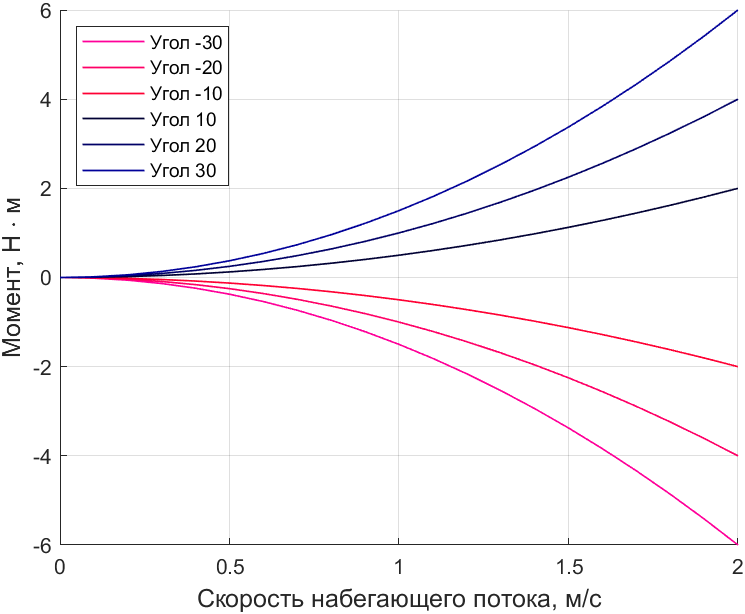
\includegraphics[width=0.8\linewidth]{modelling/Моделирование - рули скорость.png}
    \caption{Численное моделирование момента создаваемого рулем управления при различных скоростях набегающего потока.}
    \label{fig:modelling-rudder-velocity}
\end{figure}

\section{Выводы по 2}
